
\documentclass[english,12pt,a4paper,pdftex]{article}
%% This package is required
%% Choose your school from arts, biz, chem, elec, eng, sci.
%% Choose the character encoding scheme used by your editor: utf8, latin1

\usepackage[elec,utf8]{aaltothesis} % this is the default in aaltothesis.sty
%% Use this if you run pdflatex and use jpg/pdf-format pictures.

\usepackage{graphicx}

%% Use the macros in this package to change how the hyperref package below 
%% typesets its hypertext -- hyperlink colour, font, etc. See the package
%% documentation. It also defines the \url macro, so use the package when 
%% not using the hyperref package.
%\usepackage{url}

%% Use this if you want to get links and nice output with pdflatex
\usepackage[pdfpagemode=None,colorlinks=true,urlcolor=red,%
linkcolor=blue,citecolor=black,pdfstartview=FitH]{hyperref}

%% Use this if you write hard core mathematics, these are usually needed
\usepackage{amsfonts,amssymb,amsbsy}  

%% Horizontal margins, DO NOT TOUCH!
\setlength{\hoffset}{-1in}
\setlength{\oddsidemargin}{35mm}
\setlength{\evensidemargin}{25mm}
\setlength{\textwidth}{15cm}
%% Vertical margins, DO NOT TOUCH!
\setlength{\voffset}{-1in}
\setlength{\headsep}{7mm}
\setlength{\headheight}{1em}
\setlength{\topmargin}{25mm-\headheight-\headsep}
\setlength{\textheight}{23cm}

%% Output starts here
\begin{document}
%% Change the school field to describe your school if the autimatically 
%% set name is wrong
% \university{aalto University}{aalto-Yliopisto}
% \school{School of Electrical Engineering}{SähköTekniikan korkeakoulu}

%% Vain kandityölle: Korjaa seuraavat vastaamaan koulutusohjelmaasi
%%
%% Only for B.Sc. thesis: Choose your degree programme. 
%\degreeprogram{Electronics and electrical engineering}%

%% Only for M.Sc. and Licentiate thesis: Choose your department,
%% professorship and professorship code. 
\department{Department of Signal Processing and Acoustics}%
{Signaalinkäsittelyn ja akustiikan laitos}
\professorship{Speech and Language Processing}{}
\code{S-89}

%% Choose one of these:
%\univdegree{BSc}
%\univdegree{MSc}
%% Added by Jose: For the non-finnish/swedish, the Lic degree is half of a PhD.
%\univdegree{Lic}
%% Add by Jose: For engineering exchange students (old plan, not Bolonia), PFC in Spain
%% IMPORTANT: FPr is only valid with English!!!
\univdegree{FPr}
%% Should be self explanatory...
\author{Jose Mariano Moreno Pimentel}

%% Your thesis title. If the title is very long and the latex 
%% does unsatisfactory job of breaking the lines, you will have to
%% break the lines yourself with \\ control character. 
%% Do not hyphenate titles.
\thesistitle{Text-to-Speech adaptation using noisy data}{}

\place{Espoo}
%% For B.Sc. thesis use the date when you present your thesis. 
\date{31.03.2014}

%% B.Sc. or M.Sc. thesis supervisor 
%% Note the "\" after the comma. This forces the following space to be 
%% a normal interword space, not the space that starts a new sentence. 
\supervisor{Prof.\ Mikko Kurimo}{Prof.\ Mikko Kurimo}

%% B.Sc. or M.Sc. thesis advisors(s). 
%%
%% Note that there has been a change in the official EN translation
%% of the Finnish title ``ohjaaja'' which in the previous version (1.5) 
%% of this document was called ``instructor''. The recommended
%% translation is now ``advisor''.  
%% However, the LaTeX internal variable remains \instructor
%% as there is little point to change the variable name. 
%%
%\instructor{Prof. Pirjo Professori}{Prof. Pirjo Professori}
%\instructor{D.Sc.\ (Tech.) Olli Ohjaaja}{TkT Olli Ohjaaja}
\instructor{M.Sc.\ (Tech.) Reima Karhila}{DI Reima Karhila}

%% Aalto logo: syntax:
% \uselogo{aaltoRed|aaltoBlue|aaltoYellow|aaltoGray|aaltoGrayScale}{?|!|''}
%% Logo language is set to be the same as the document language.
\uselogo{aaltoBlue}{''}

%% Create the coverpage
\makecoverpage

%% Force new page so that English abstract starts from a new page
\newpage
%
%% English abstract, uncomment if you need one. 
%% 
%% Abstract keywords
\keywords{speech synthesis, synthetic speech, TTS, HMM, noise robust, TTS adaptation}
%% Abstract text
\begin{abstractpage}[english]
 Your abstract in English. Try to keep the abstract short, approximately 
 100 words should be enough. Abstract explains your research topic, 
 the methods you have used, and the results you obtained.  
\end{abstractpage}
%% Note that 
%% if you are writting your master's thesis in English place the English
%% abstract first followed by the possible Finnish abstract

%% Preface
%\mysection{Esipuhe}
\mysection{Acknowledgments}

\vspace{5cm}
Otaniemi, 24.9.2013

\vspace{5mm}
{\hfill Jose M.\ Moreno \hspace{1cm}}

%% Force new page after preface
\newpage

%% Table of contents. 
\thesistableofcontents

\newpage
%% List of figures
\listoffigures

\newpage
%% List of tables
\listoftables

%% Symbols and abbreviations
\mysection{Symbols and abbreviations}
\subsection*{Symbols}

\subsection*{Opetators}

\subsection*{Abbreviations}
\begin{tabular}{ll}
	HMM			& Hidden Markov Model\\
	LPC 			& Linear Predictive Coding\\
	LSP			& Line Spectral Pair\\
	STRAIGHT	& Speech Transformation and Representation using Adaptive \\
				& Interpolation of weiGHT spectrum\\
	TTS			& Text-To-Speech
\end{tabular}
%% Corrects the page numbering, there is no need to change these
\cleardoublepage
\storeinipagenumber
\pagenumbering{arabic}
\setcounter{page}{1}

\section{Introduction}
\label{intro}
\thispagestyle{empty}

Speech synthesis is not a recent ambition in mankind history. The earliest attempts to synthesize speech are only legends starring Gerbert d'Aurillac (died 1003 A.D.), also known as Pope Sylvester II. The pretended system used by him was a brazen head: a legendary automaton imitating the anatomy of a human head and capable to answer any question. Back in those days, the brazen heads were said to be owned by wizards. Following Pope Sylvester II, some important characters in mankind history  were reputed to have one of these heads, such as Albertus Magnus or Roger Bacon.

During the 18th century, Christian Kratzenstein, a German-born doctor, physicist and engineer working at the Russian Academy of Sciences, was able to built acoustics resonators similar to the human vocal tract. He activated the resonators with vibrating reeds producing the the five long vowels: /a/, /e/, /i/, /o/ and /u/.

Almost at the end of the 18th century, in 1791, Wolfgang von Kempelen presented his Acoustic-Mechanical Speech Machine \cite{vonKempelen}, which was able to produce single sounds and some combinations. During the first half of the 19th century, Charles Wheatstone built his improved and more complicated version of Kempelen's Acoustic-Mechanical Speech Machine, capable of producing vowels, almost all the consonants, sound combinations and even some words.	

In the late 1800's, Alexander Graham Bell also built a speaking machine and did some questionable experiments changing with his hands the vocal tract of his dog and making the dog bark in order to produce speech-like sounds \cite{Schroeder93}.


\section{History of Speech Synthesis}
\label{history_speech_synthesis}
Speech synthesis can be defined as the artificial generation of speech. Nowadays the process has been facilitated due to the improvements made during the last 70 years in computer technology, making the computer-based speech synthesis systems lead the way supported by their flexibility and their easier access compared to mechanical systems. However, after the first resonators built by Kratzenstein, the fist speaking machine was built and presented to the world in 1791, and was obviously mechanic.

\subsection{Acoustical-Mechanical Speech Machines}
The speech machine developed by von Kempelen incorporated models of the lips and the tong, enabling it to produce some consonants as well as vowels. Although Kratzenstein presented his resonators before von Kempelen his speech machine, von Kempelen started his work quite before, publishing a book where he described the studies made on human speech production and the experiments he made with his speech machine over 20 years of work \cite{vonKempelen}.  

The machine was composed by a pressure chamber, acting as lungs, a vibrating reeds in charge of the functions of the vocal cords and a leather tube that was manually manipulated in order to change its shape as the vocal tract does in an actual person, producing different vowel sounds. It had four separate constricted passages, controlled by the fingers, to generate consonants. Von Kempelen also included in his machine a model of the vocal tract with a hinged tongue and movable lips so as to create plosive sounds \cite{Schroeder93, LemmettyMSc, flanagan_1973_speech}. 



\begin{figure}[htb]
	\begin{center}
		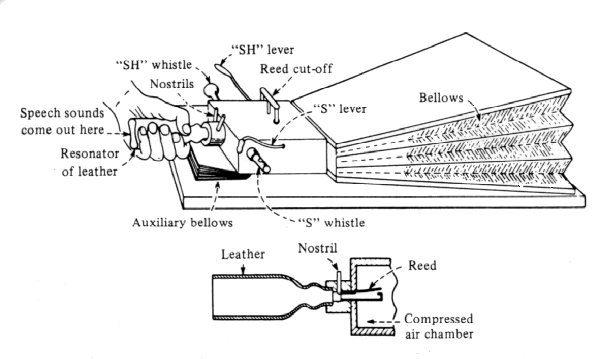
\includegraphics[width=\textwidth]{images/von_kempelen_machine.jpg}
		\caption{\cite{flanagan_book}}
	\end{center}
\end{figure}
%\section{Introduction}

%% Leave first page empty
%\thispagestyle{empty}

%% In a thesis, every section starts a new page, hence \clearpage
%\clearpage



%% Three levels of hierarchy in sectioning should be enough

\clearpage

%% The \phantomsection command is nessesary for hyperref to jump to the 
%% correct page, in other words it puts a hyper marker on the page.

\phantomsection
%\addcontentsline{toc}{section}{Viitteet}
\addcontentsline{toc}{section}{References}
\bibliographystyle{ieeetr}
\bibliography{sections/references}



\appendix 
\clearpage
%% Adds the word "Appendices" to the table of contents
\addtocontents{toc}{\protect\contentsline{section}{Appendices}{}{appendix}}

 %% appendix example (starts with section) in Finnish

%% Equations, tables and figures have their own numbering in Appendices, REMEMBER TO DO EVERY TIME YOU START AN APPENDIX, THE LETTER A IS THE APPENDIX INDEX
\renewcommand{\theequation}{A\arabic{equation}}
\setcounter{equation}{0}  
\renewcommand{\thefigure}{A\arabic{figure}}
\setcounter{figure}{0}
\renewcommand{\thetable}{A\arabic{table}}
\setcounter{table}{0}


\end{document}
